\begin{frame}{Problema: sinais não mudam instantaneamente}
  \begin{itemize}
    \item Em circuitos reais, cada porta lógica possui atraso de propagação.
    \item Um dado pode mudar perto da borda do clock.
    \item Se o destino ler cedo ou tarde demais, poderá receber valor incorreto.
  \end{itemize}
  \vspace{0.15cm}
  \begin{center}
  \resizebox{0.9\linewidth}{!}{%
  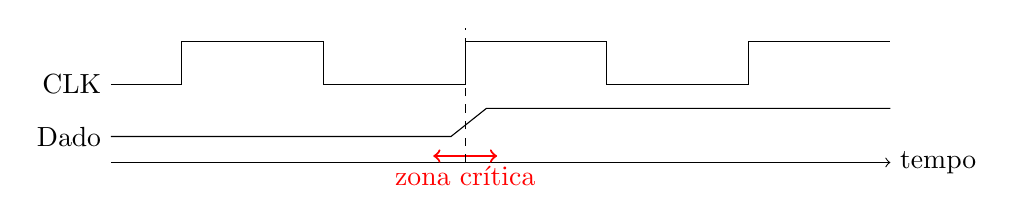
\begin{tikzpicture}[x=0.9cm,y=0.55cm]
    \draw[->] (0,0) -- (11,0) node[right]{tempo};
    \draw (0,1.8) node[left]{CLK} -- (1,1.8)--(1,2.8)--(3,2.8)--(3,1.8)--(5,1.8)--(5,2.8)--(7,2.8)--(7,1.8)--(9,1.8)--(9,2.8)--(11,2.8);
    \draw (0,0.6) node[left]{Dado} -- (4.8,0.6)--(5.3,1.25)--(11,1.25);
    \draw[red, thick, <->] (4.55,0.15)--(5.45,0.15) node[midway,below]{zona crítica};
    \draw[dashed] (5,0) -- (5,3.1);
  \end{tikzpicture}%
  }
  \end{center}
\end{frame}